\documentclass[12pt]{article}
\usepackage{amsmath}
\usepackage{physics}
\usepackage{graphicx}
\usepackage[linesnumbered,ruled,vlined]{algorithm2e}
\author{Patryk Kozlowski}
\title{G0W0}
\date{\today}
\begin{document}
\maketitle
\section{Notation}
$p,q,r,s,...$ are used for general orbitals. $i,j,k,l,...$ are used for occupied orbitals. $a,b,c,d,...$ are used for virtual orbitals. We write our spatial integrals in the chemists notation as:
\begin{equation}
    (pq|rs) = \int \int \frac{\phi _{p}^{*}(r_{1}) \phi _{q}(r_{1}) \phi _{r}^{*}(r_{2}) \phi _{s}(r_{2})}{r_{12}} \dd r _{1} \dd r _{2}
\end{equation}
\section{Self Energy}
First, we are interested in implementing the diagonal of the real part of the correlation part of the self-energy. This is given by:
\begin{equation}
    \Sigma_{pp}^{\text{correlation}}(\omega) = \sum_{\mu }^{\text{RPA}}\left(\sum_{j}^{\text{occupied}} \frac{V_{pj}^{\mu }V_{pj}^{\mu }}{\omega -(\varepsilon _{j}-\Omega  _{\mu })}+ \sum_{b}^{\text{virtual}} \frac{V_{pb}^{\mu }V_{bp}^{\mu }}{\omega -(\varepsilon _{b}+\Omega  _{\mu })}\right)
\end{equation}
Most of the entities are known, so we first turn our attention to the $V$ and $\Omega_{\mu }$. The derivation of these quantities will be made in the Tamm-Dancoff approximation of the RPA. First, we consider the tensor $A$:
\begin{equation}
    A_{iajb}=\delta _{ij} \delta _{ab} \left(\varepsilon _{a}-\varepsilon _{i}\right) + (\underline{i} \underline{a} | \underline{j} \underline{b} )
\end{equation}
The underlines within the two-electron integral are being used to emphasize that these are spin indices and not spatial indices yet. In order for the integral not to vanish, the first and the second pairs of indices need to have the same spin. \emph{Furthermore, the total spin must be conserved.} Now, it should be mentioned that for every spatial electron repulsion integral, there can be two possible spin orbital combinations following the previous rules:
\begin{equation}
    (ia|jb) \rightarrow (i_{\alpha }a_{\alpha }|j_{\beta }s_{\beta }) , (i_{\beta }a_{\beta }|j_{\alpha }b_{\alpha })
\end{equation}
So, the factor is 2. We can now write the tensor as:

\begin{equation}
    A_{iajb}=\delta _{ij} \delta _{ab} \left(\varepsilon _{a}-\varepsilon _{i}\right) + 2(ia|jb)
\end{equation}
\emph{From what you said on Tuesday, I assume that this factor probably should be a 4.\\}We can then reshape this tensor into a matrix:
\begin{equation}
    A_{iajb} \rightarrow A_{\mu ,\nu }
\end{equation}
Where $\mu$ is a combination of $i$ and $a$ and $\nu$ is a combination of $j$ and $b$.
For the sake of a clearer understanding, we will write out a summation of the eigenvalue problems:
\begin{equation}
    \sum_{jb} \textbf{A}_{ia,jb} \textbf{R}_{jb,n} = \textbf{R}_{ia,n} \textbf{E}
\end{equation}


At this point, one can recognize that the combination of $ia$ represents a series of excitations $\mu $. There are nocc x nvirt of these. Likewise, we will represent the combination of $jb$ by the index $\nu $. $\textbf{E}$ is a diagonal matrix of the eigenvalues $E_{n}$. We can then write:
\begin{equation}
    \sum_{\nu} \textbf{A}_{\mu ,\nu } \textbf{R}_{\nu, n} = \textbf{R}_{\mu ,n} \textbf{E}
\end{equation}
\emph{What is the tda. does it end here or continue into the W?\\}
For a given excitation, we already have the $\Omega $/E, but we need to find the $V$.
First, we consider a tensor of dimension 4:
\begin{equation}
    W_{p,q,i,a} = \sum_{\underline{p,q,i,a}} (\underline{p} \underline{q} | \underline{i} \underline{a} )
\end{equation}
Again, our conversion from spin to spatial integrals will give a factor of $4$:
\begin{equation}
    W_{p,q,i,a} = 4 \sum_{p,q,i,a} (pq|ia)
\end{equation}
We can then reshape this tensor:
\begin{equation}
    W_{p,q,i,a} \rightarrow W_{p,q, \mu }
\end{equation}
Where $\mu$ is a combination of $i$ and $a$. We can then use the eigenvectors to get the $V$:
\begin{equation}
    V_{p,q,n} = \sum_{\mu } W_{p,q,\mu } R_{\mu ,n }
\end{equation}
\section{Self Consistent Equation}
Now that we have the real part of the correlation self-energy for a given orbital, we can incorporate it into a self-consistent procedure to obtain quasiparticle energies. The self-consistent equation is given by:
\begin{equation}
    \delta_{pq}F_{pq}^{HF}[\gamma^{DFT/HF }] + \Sigma_{p}^{corr}(\varepsilon_{p}^{QP}) = \varepsilon_{p}^{QP}
\end{equation}
\subsection{Fock Matrix with the HF Electron Density}
My understanding is that this is going to be easier to start with.
\subsection{Solving the iterative equation}
We can iteratively solve this equation. First, we have:
\begin{equation}
   \omega \equiv  \varepsilon_{p}^{QP} = \varepsilon_{p}^{DFT}
\end{equation}
\newpage
Also, graphically we can see that:
\begin{figure}[h]
    \centering
    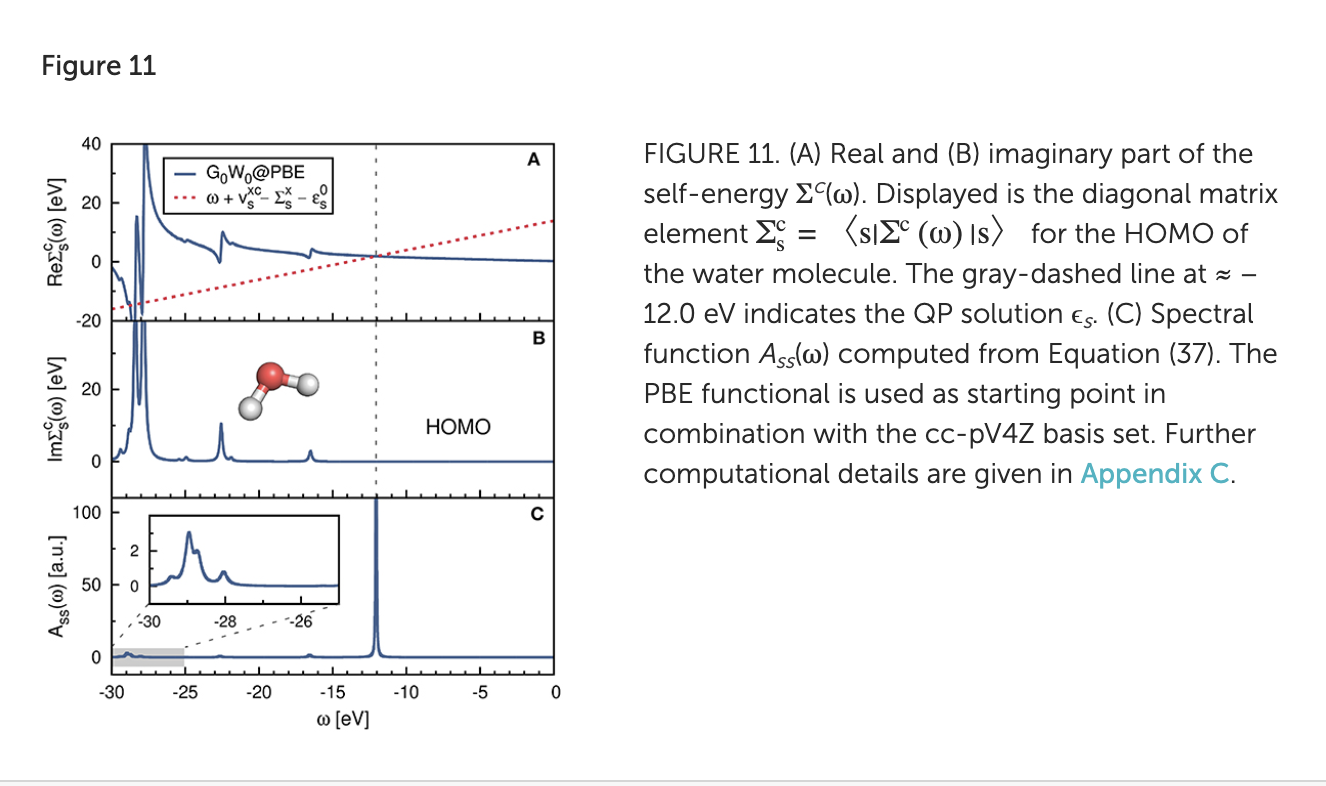
\includegraphics[width=\textwidth]{water.png}
    \caption{Graphical representation of the self-consistent equation.}
    \label{fig:my_label}
\end{figure}
My current understanding is if we think about the quantity $\omega + v_{s}^{xc}- \Sigma _{s}^{x}- \varepsilon _{s}^{0}$ this is similar to when we had:
\begin{equation}
    \varepsilon _{p}+\Sigma _{p}^{corr}(\omega )=\omega \rightarrow \Sigma _{p}^{corr}(\omega ) = \omega -\varepsilon _{p}^{QP}
\end{equation}
In the above equation $-\varepsilon _{p}^{QP}$ is analalogous to the $v_{s}^{xc}- \Sigma _{s}^{x}- \varepsilon _{s}^{0}$ that they have?
So this is simply something like $y=x-b$. Are you able to explain what exactly is meant here by obtaining a "graphical" solution?
\end{document}